\documentclass[tikz,border=3.14mm]{standalone}
\begin{document}
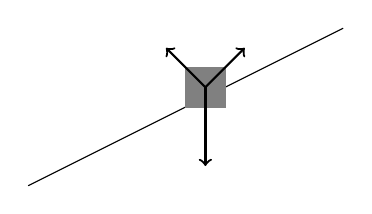
\begin{tikzpicture}
    % Draw the inclined plane
    \draw (0,0) -- (4,2);
    
    % Draw the block
    \filldraw [gray] (2,1) rectangle (2.5,1.5);
    
    % Draw the three forces: gravity, normal force, and friction.
    % Gravity
    \draw [thick,->] (2.25,1.25) -- (2.25,0.25);
    % Normal force
    \draw [thick,->] (2.25,1.25) -- (1.75,1.75);
    % Friction force
    \draw [thick,->] (2.25,1.25) -- (2.75,1.75);
\end{tikzpicture}
\end{document}